\documentclass[12pt,a4paper]{article}

% Paquetes de configuración del documento
\usepackage[utf8]{inputenc}
\usepackage[spanish]{babel}
\usepackage[T1]{fontenc}
\usepackage[margin=2.5cm]{geometry}
\usepackage{fancyhdr}
\usepackage{siunitx}
%Paquetes para simbologia%
\usepackage{amsmath}
\usepackage{amsfonts}
\usepackage{amssymb}
\usepackage{physics}
\usepackage{longtable}
\usepackage{graphicx}
\usepackage{caption}
\usepackage{float}
\usepackage{xurl}
\usepackage[colorlinks=true,
            linkcolor=black,
            urlcolor=myblue,
            citecolor=black,
            filecolor=black]{hyperref}
 % Opción estándar para enlaces
\Urlmuskip=0mu plus 1mu          % Mejora el espaciado para permitir cortes
\usepackage{subcaption}  % en el preámbulo
\usepackage{pgfplots}
\pgfplotsset{compat=1.18}
\usepackage{tikz}
\usepackage{xcolor}
\definecolor{myblue}{RGB}{42, 127, 179}

\pagestyle{fancy}
\chead{\textit{Materiales Metálicos}}
\rhead{\textit{UTN-FRVM}}
\lhead{\textit{Ingeniería Mecánica}}

\begin{document}
\begin{titlepage}
	
	\begin{center}
		{\huge \textit{Universidad Tecnológica Nacional}}\\
        \vspace{0.5cm}
		{\LARGE \textit{Facultad Regional Villa María}}\\
		\vspace{1.5cm}
        {\LARGE{\textit{Ingeniería Mecánica - Materiales Metálicos}}}\\
		\vspace{1.5cm}
        \LARGE{\textit{Trabajo Práctico 3-06}}
	\end{center}
	
	\vfill

    \textit{Grupo DEL RÍO:}
	\begin{itemize}
		\item \textit{Abregú, Iván.}
		\item \textit{Antico, Rodrigo.}
		\item \textit{Brussa,Julián.}
		\item \textit{Cabral, Franco.}
        \item \textit{Cárdenas, Felipe.}
        \item \textit{Cardozo, Martín.}
        \item \textit{Córdoba, Nathan.}
        \item \textit{Cucco, Ramiro.}
        \item \textit{del Río, Juan.}
        \item \textit{Guerini, Nazareno.}
        \item \textit{Medina, Ivo.}
        \item \textit{Ortiz, Gastón.}
        \item \textit{Picos, Elías.}
        \item \textit{Quinteros, Lautaro.}
	\end{itemize}
    
	\textit{Docentes:}
	\begin{itemize}
		\item \textit{Dr. Lucioni, Eldo José.}
		\item \textit{Ing. Victorio Vallaro, Juan Manuel.}
	\end{itemize}
	\centering
	\today
	
\end{titlepage}

\newpage
\tableofcontents

\begin{abstract}
    \begin{itemize}
        \item Tamaño de grano.
        \item Micrografía.
        \item Relación resistencia-dureza.
        \item Relación resistencia-tamaño de grano.
        \item Carbono Equivalente (CE) y Parámetro Crítico del Material (PCM).
        \item Soldabilidad.
        \item Deslizamiento de dislocaciones y de grano.
    \end{itemize}
    
    \underline{\textbf{REQUERIMIENTOS:}}

    \begin{itemize}
        \item Tomar imágenes metalográficas de la probeta en el laboratorio de materiales de la facultad en los puntos indicados para  cada equipo (la probeta se  entregara pulida con alúmina, cada equipo debe decidir el reactivo para el ataque y el tiempo de ataque.)
        \item Obtener el valor de resistencia para la muestra usando el modelo físico matemático de Hall-Petch (ORIENTACIÓN 001).
        \item Obtener el valor de dureza para la muestra usando la extensión del modelo físico matemático de Hall-Petch  (ORIENTACIÓN 001).
        \item Determinar la soldabilidad de cada uno de los materiales empleando las expresiones de la American Welding Society (AWS) y del Instituto Internacional de Soldadura (IIW). (ORIENTACIÓN 002).
        \item Analizar la soldabilidad de los materiales y las diferencias que se ven en la macrografía provista. (ORIENTACION 3).
        \item ¿Para qué se usa el parámetro crítico del metal (Pcm) adoptado por la Sociedad Japonesa de Ingeniería de Soldadura? ¿Cuál es su expresión? (No es necesario que efectúe el cálculo).
        \item Calcular la resistencia a la tracción a partir de los modelos empíricos que relacionan resistencia con dureza.  (ORIENTACIÓN 4).
        \item Analizar la presencia del fenómeno de deslizamiento de dislocación versus el fenómeno de deslizamiento de borde de grano. (ORIENTACIÓN 5).
    \end{itemize}

    \underline{\textbf{DATOS:}}

    \begin{itemize}
        \item Cada equipo debe seleccionar un punto e informar su decisión por correo, no pueden existir dos equipos con el mismo punto A, B, C, D.
        \item Imagen:
        \begin{figure}[h]
            \centering
            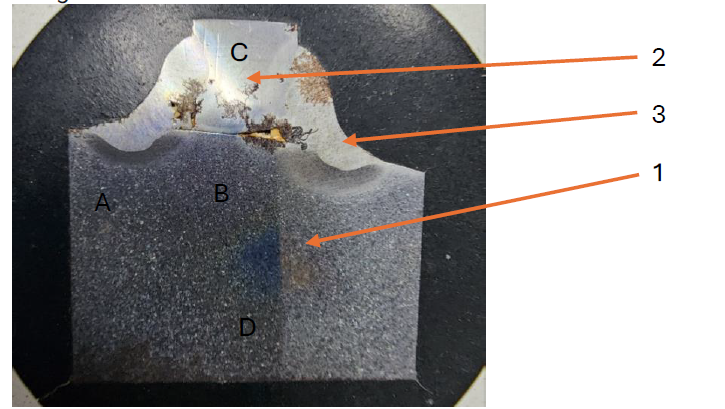
\includegraphics[width=0.5\linewidth]{Figuras/imagen 1.png}
            \label{figura1}
        \end{figure}
        \item Composición química material 1:
            \begin{table}[h]
                \centering
                \begin{tabular}{|l|l|l|l|l|l|l|l|}
                C\%   & Si\%  & Mn\%  & P\%   & S\%   & Cr\%  & Mo\%  & Ni\%  \\
                0,455 & 0,231 & 0,745 & 0,005 & 0,003 & 0,041 & 0,007 & 0,037
                \end{tabular}
            \end{table}
        \item Composición del material 2: acero IRAM 1020.
        \item Composición del material aporte, web: \href{https://esab.com/ar/sam_es/products-solutions/product/filler-metals/mild-steel/mig-wires-tig-rods-gmaw-gtaw/ok-autrod-12-51/}{esab-ok-autrod-12-51/}
        \item \(\textit{HV}_0=\) obtenerla con el durómetro en la zona no tratada.
        \item \(\sigma_0=\) obtenerlo de la hoja técnica del acero que corresponda por hoja técnica.
        \item \(d=\) medirla con el microscopio.
        \item modelo físico matemático:
        \item \(\sigma_y=\) usar el modelo de Hall Petch.
        \item \(\textit{HV}_0=\) usar el dato medido en alguno de los durómetros del laboratorio.
    \end{itemize}

    \underline{\textbf{ORIENTACIONES:}}

    \underline{\textbf{ORIENTACIÓN 001: Emplear la técnica del paper de referencia:}}

    \begin{itemize}
        \item Artículo científico:  Baker, B.; Menon, E.; Mcnelley, T.; Brewer, L.; El-Dasher, B.; Farmer, Joseph, C.; Torres, S.; Mahoney, M.; Sanderson, S. (2014). Processing-Microstructure Relationships in Friction Stir Welding of MA956 Oxide Dispersion Strengthened Steel. Metallurgical and Materials Transactions E. 1. 1-13. DOI: \href{http://dx.doi.org/10.1007/s40553-014-0033-6}{10.1007/s40553-014-0033-6}. Sitio Web: \href{https://www.researchgate.net/publication/305807425_Processing-Microstructure_Relationships_in_Friction_Stir_Welding_of_MA956_Oxide_Dispersion_Strengthened_Steel#fullTextFileContent}{researchgate}.
        \item Último párrafo de la Sección IV + la Figura 14:\\
        Cuando los datos de dureza actuales se trazan frente a la raíz cuadrada inversa del tamaño de grano del material de la zona de agitación, se observa una gráfica relativamente lineal para cuatro de las condiciones de FSW (Figura 14). Esta relación lineal sugiere la relación Hall-Petch que describe la conexión entre el tamaño del grano y el límite elástico en materiales cristalinos. Por el contrario, la dureza del material base es mucho mayor y no cae en esta línea de regresión lineal. Se reconoce que la dureza es una medida de la resistencia al flujo plástico de un material y, por lo tanto, es una función tanto del límite elástico como del endurecimiento por deformación. Un trabajo reciente de Baker et al. Ha realizado experimentos reales de tracción uniaxial en material extraído de la zona de agitación. El límite elástico a temperatura ambiente del material de la zona de agitación sigue, de hecho, una relación de Hall-Petch. La principal diferencia en el límite elástico a baja temperatura entre el material base y el material de la zona de agitación; por lo tanto, se debe al engrosamiento de las partículas de itrio-óxido de aluminio en el material con la correspondiente pérdida en la fuerza de dispersión. Esta pérdida de fortalecimiento por dispersión es la razón por la que el valor de dureza del material base no cae en la línea Hall-Petch de la Figura 14. Se pueden encontrar más detalles sobre la evolución de estos óxidos y su impacto en el comportamiento a tracción del material de soldadura en otros trabajos recientes. Por Baker.
            \begin{figure}[h]
                \centering
                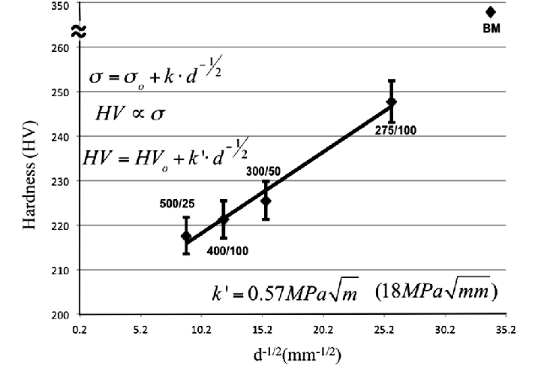
\includegraphics[width=0.5\linewidth]{figuras/imagen 2.png}
                \label{figura2}
            \end{figure}
    \end{itemize}

    \underline{\textbf{ORIENTACIÓN 002: Información de referencia.}}

    \begin{itemize}
        \item Contenido de Carbono Equivalente. Sitio Web: \href{https://academia-lab.com/enciclopedia/contenido-de-carbono-equivalente/}{academia-lab}.
    \end{itemize}

    \underline{\textbf{ORIENTACIÓN 003: Información de referencia:}}

    \begin{itemize}
        \item Anexo IV. Guía de métodos alternativos para determinar el precalentamiento en la soldadura de aceros estructurales. Sitio Web: \href{http://contenidos.inpres.gob.ar/docs/Reglamentos/CIRSOC-304-Reglamento.pdf}{contenidos.inpres}.
    \end{itemize}

    \underline{\textbf{ORIENTACIÓN 004: Información de referencia:}}

    \begin{itemize}
        \item Emplear el modelo de referencia mencionado en el artículo científico: Sáenz, P. (1989) \textit{«Cálculo para determinar la resistencia a la tracción de algunos materiales conociendo la dureza brinell y lo inverso»}, Informador Técnico, 39, pp. 16-19. Sitio Web: \href{https://revistas.sena.edu.co/index.php/inf_tec/issue/view/183/121}{revistas.sena} (pp. 16-19).
    \end{itemize} 

    \underline{\textbf{ORIENTACIÓN 005: Información de referencia:}}

    \begin{itemize}
        \item Endurecimiento del borde de grano.  Sitio Web: \href{https://es.wikipedia.org/wiki/Endurecimiento_del_borde_de_grano}{wikipedia.org} [Figura 1: El endurecimiento de Hall-Petch está limitado por el tamaño de las luxaciones. Una vez que el tamaño de grano alcanza aproximadamente 10 nanómetros, los bordes del grano comienzan a deslizarse.].
        \begin{figure}[h]
            \centering
            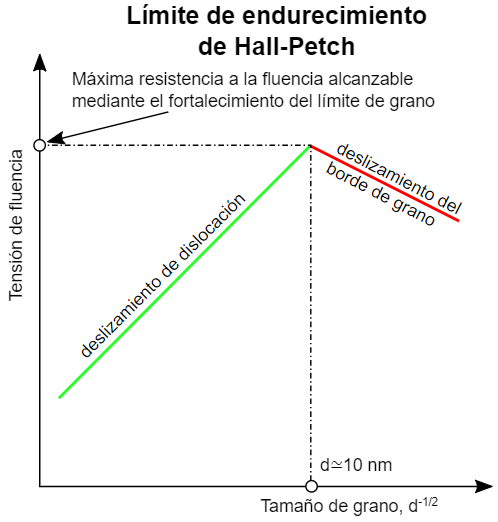
\includegraphics[width=0.5\linewidth]{figuras/imagen 3.png}
            \label{fig:enter-label}
        \end{figure}
    \end{itemize}
\end{abstract}

\section{Datos principales.}

Primero contamos con las imágenes de la pieza seleccionada, las cuales se observan en la \autoref{fig:metalografia}. En base a esto podemos obetener el diámetro promedio de los granos. Para ello empleamos "ChatGPT 4o" acompañado de un código en Python para saber cuantos granos hay en la imagen, el resultado son 613 granos como se puede ver ejecutando el código adjunto. Luego procedemos a esta herramienta nuevamente para saber cual es el diámetro promiedo de \SI{116,84}{\micro\metre}.

\begin{figure}[h!]
    \centering
    \begin{subfigure}[b]{0.45\linewidth}
        \centering
        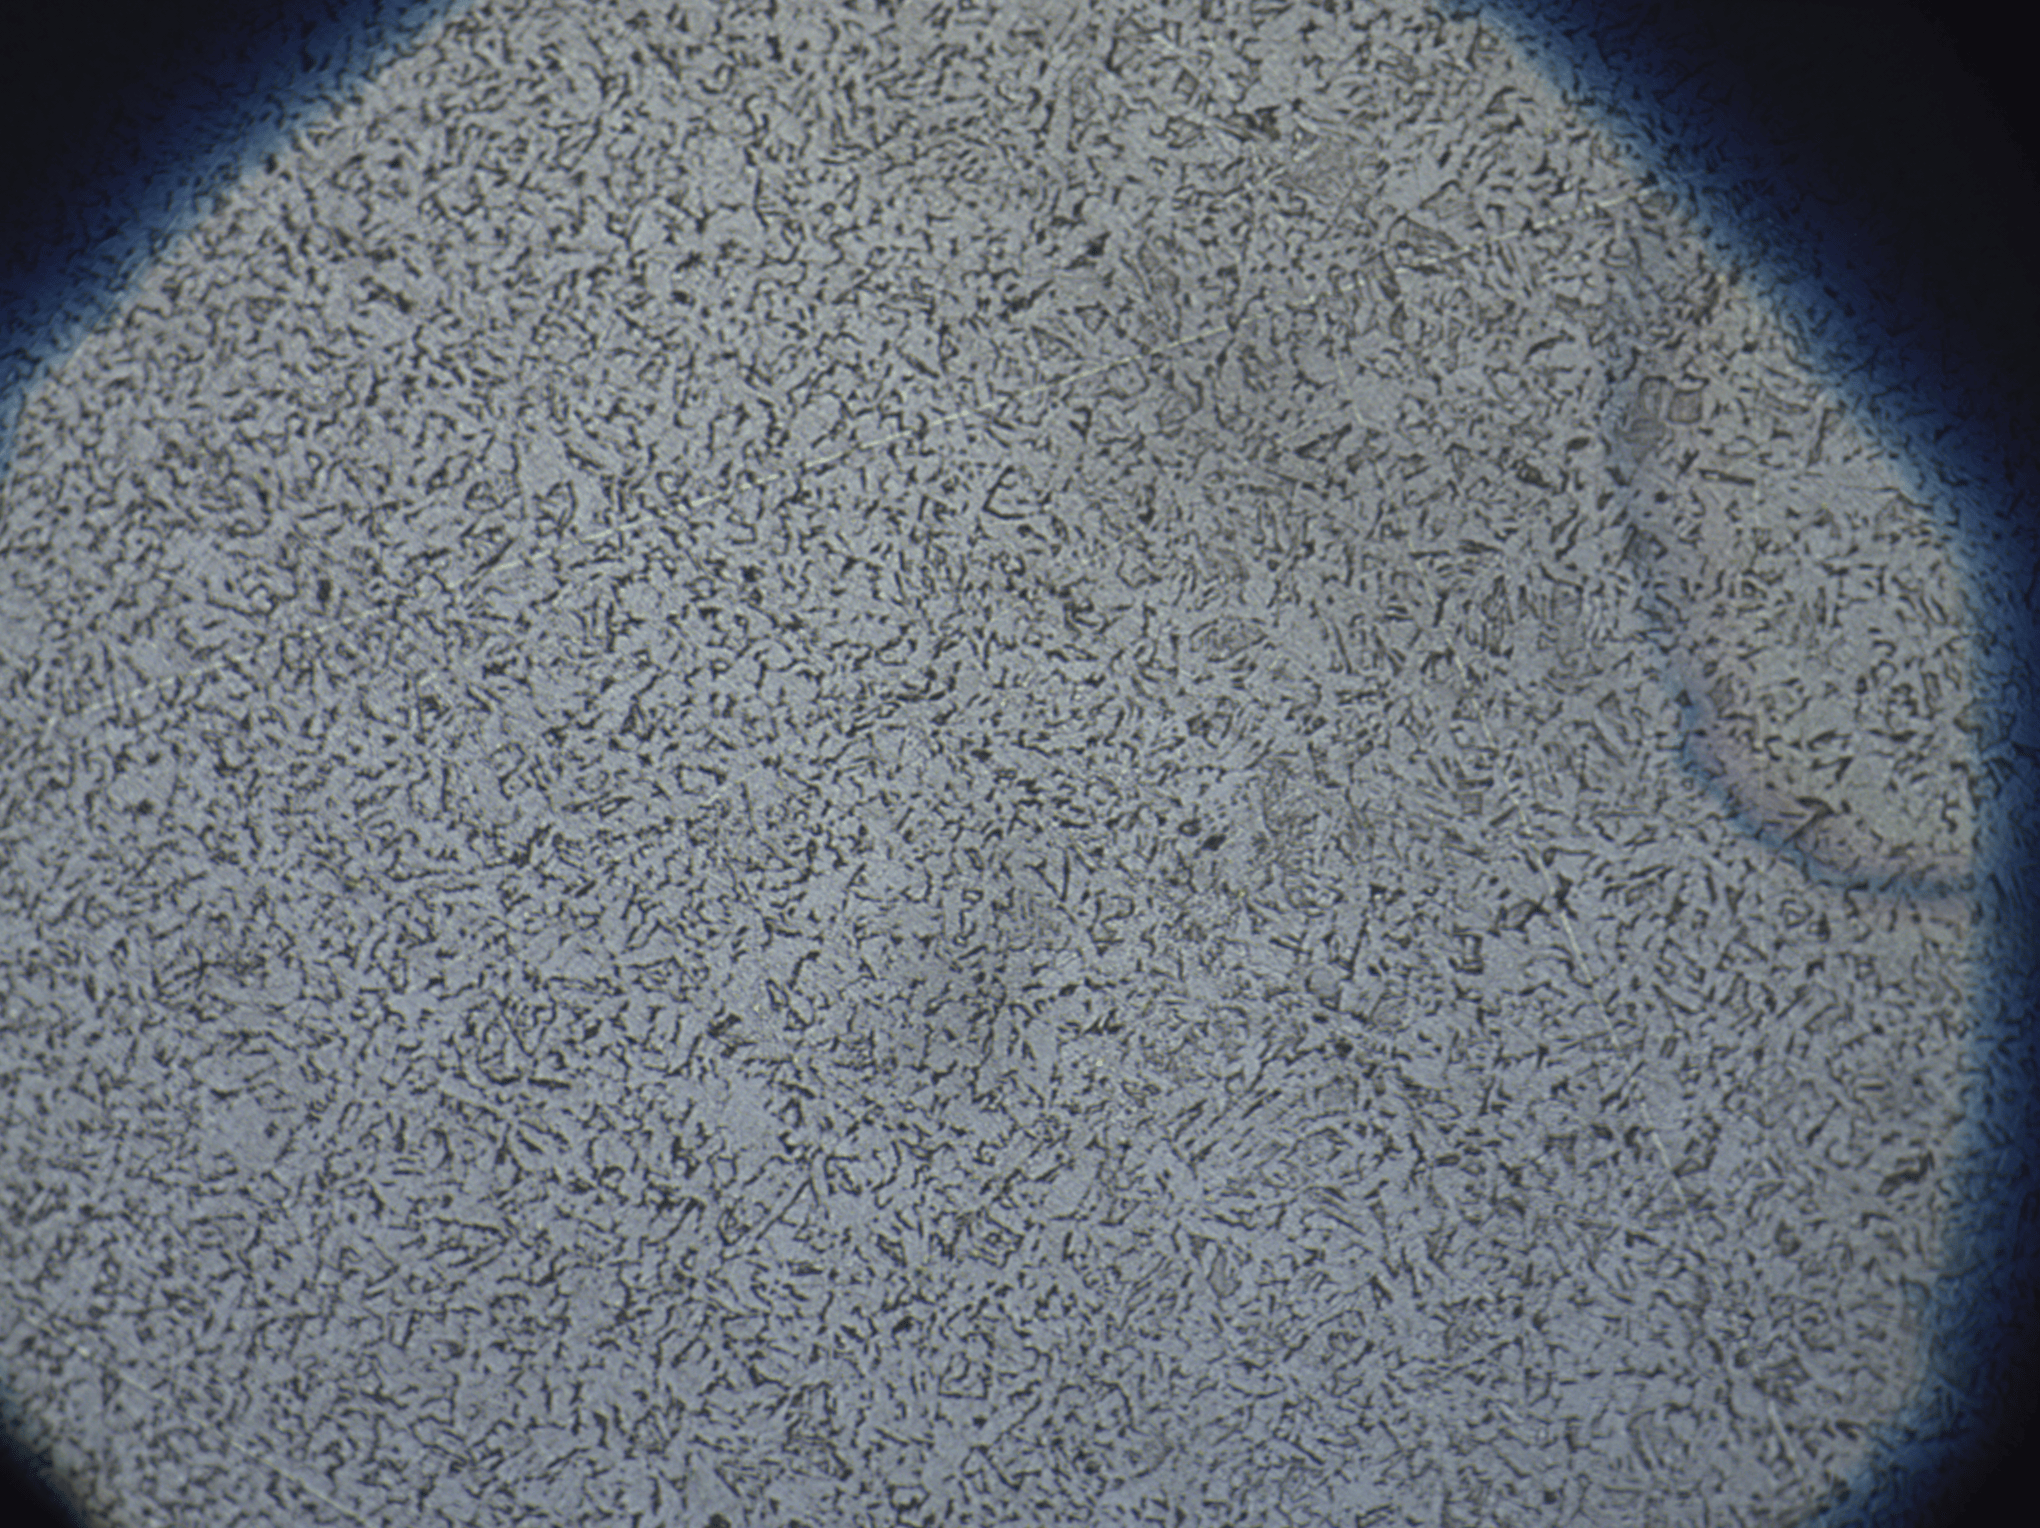
\includegraphics[width=\linewidth]{Figuras/Del-Rio_6.png}
        \caption{Acero IRAM 1020 100x.}
        \label{100x}
    \end{subfigure}
    \begin{subfigure}[b]{0.45\linewidth}
        \centering
        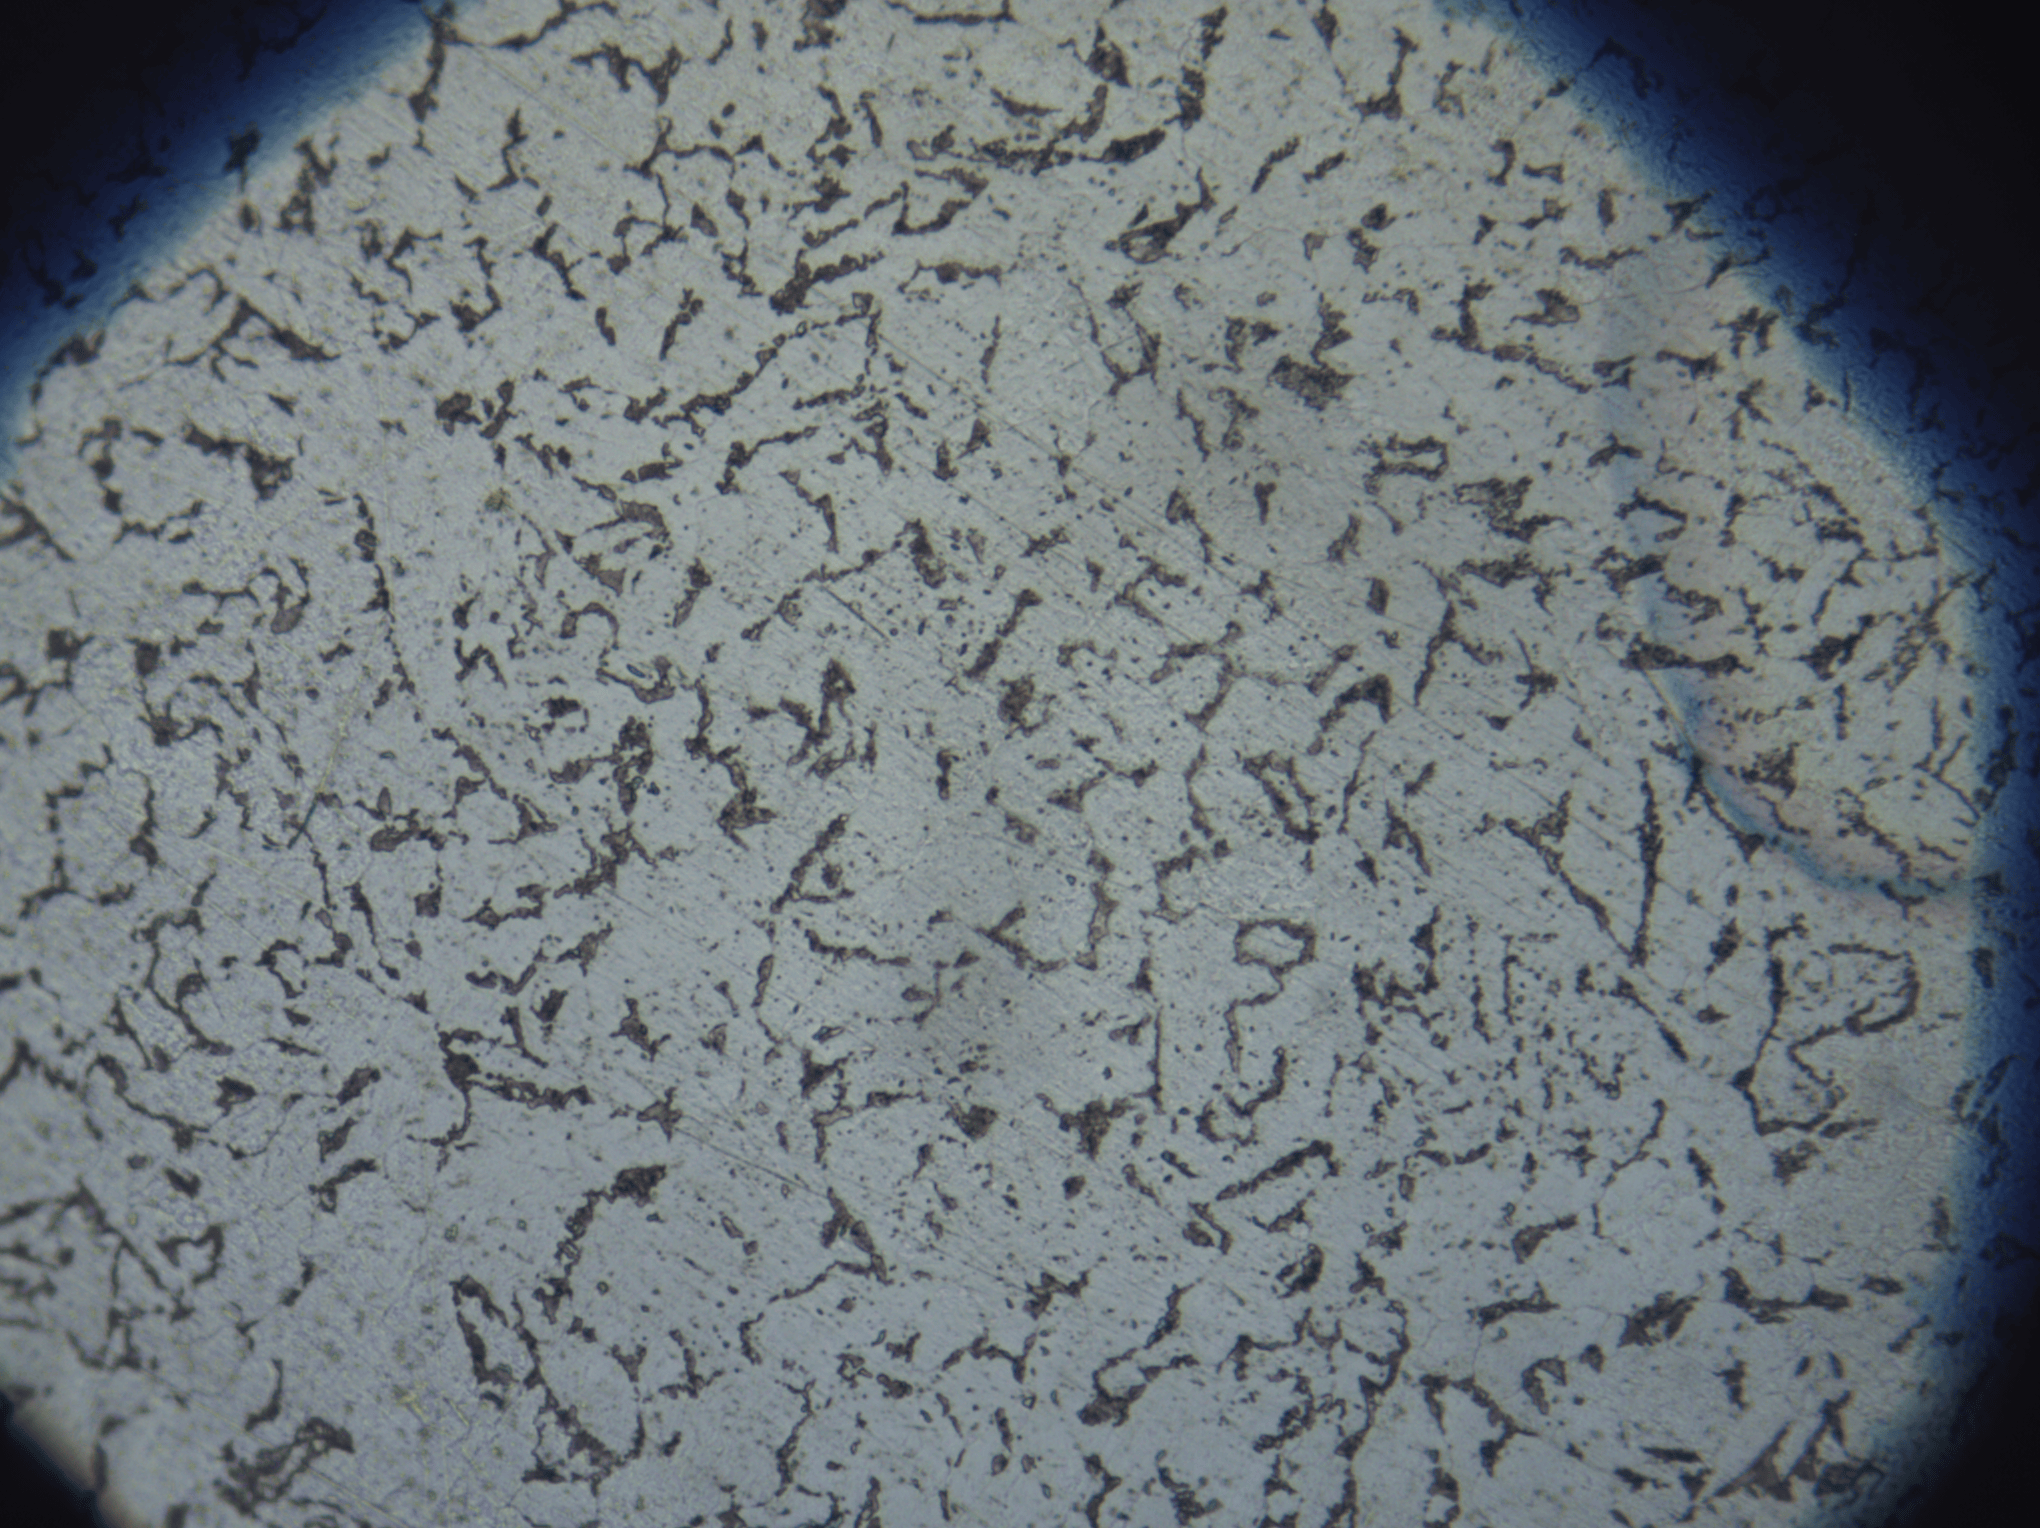
\includegraphics[width=\linewidth]{Figuras/Del-Rio_7.png}
        \caption{Acero IRAM 1020 400x.}
        \label{400x}
    \end{subfigure}

    \vspace{1em}

    \begin{subfigure}[b]{0.6\linewidth}
        \centering
        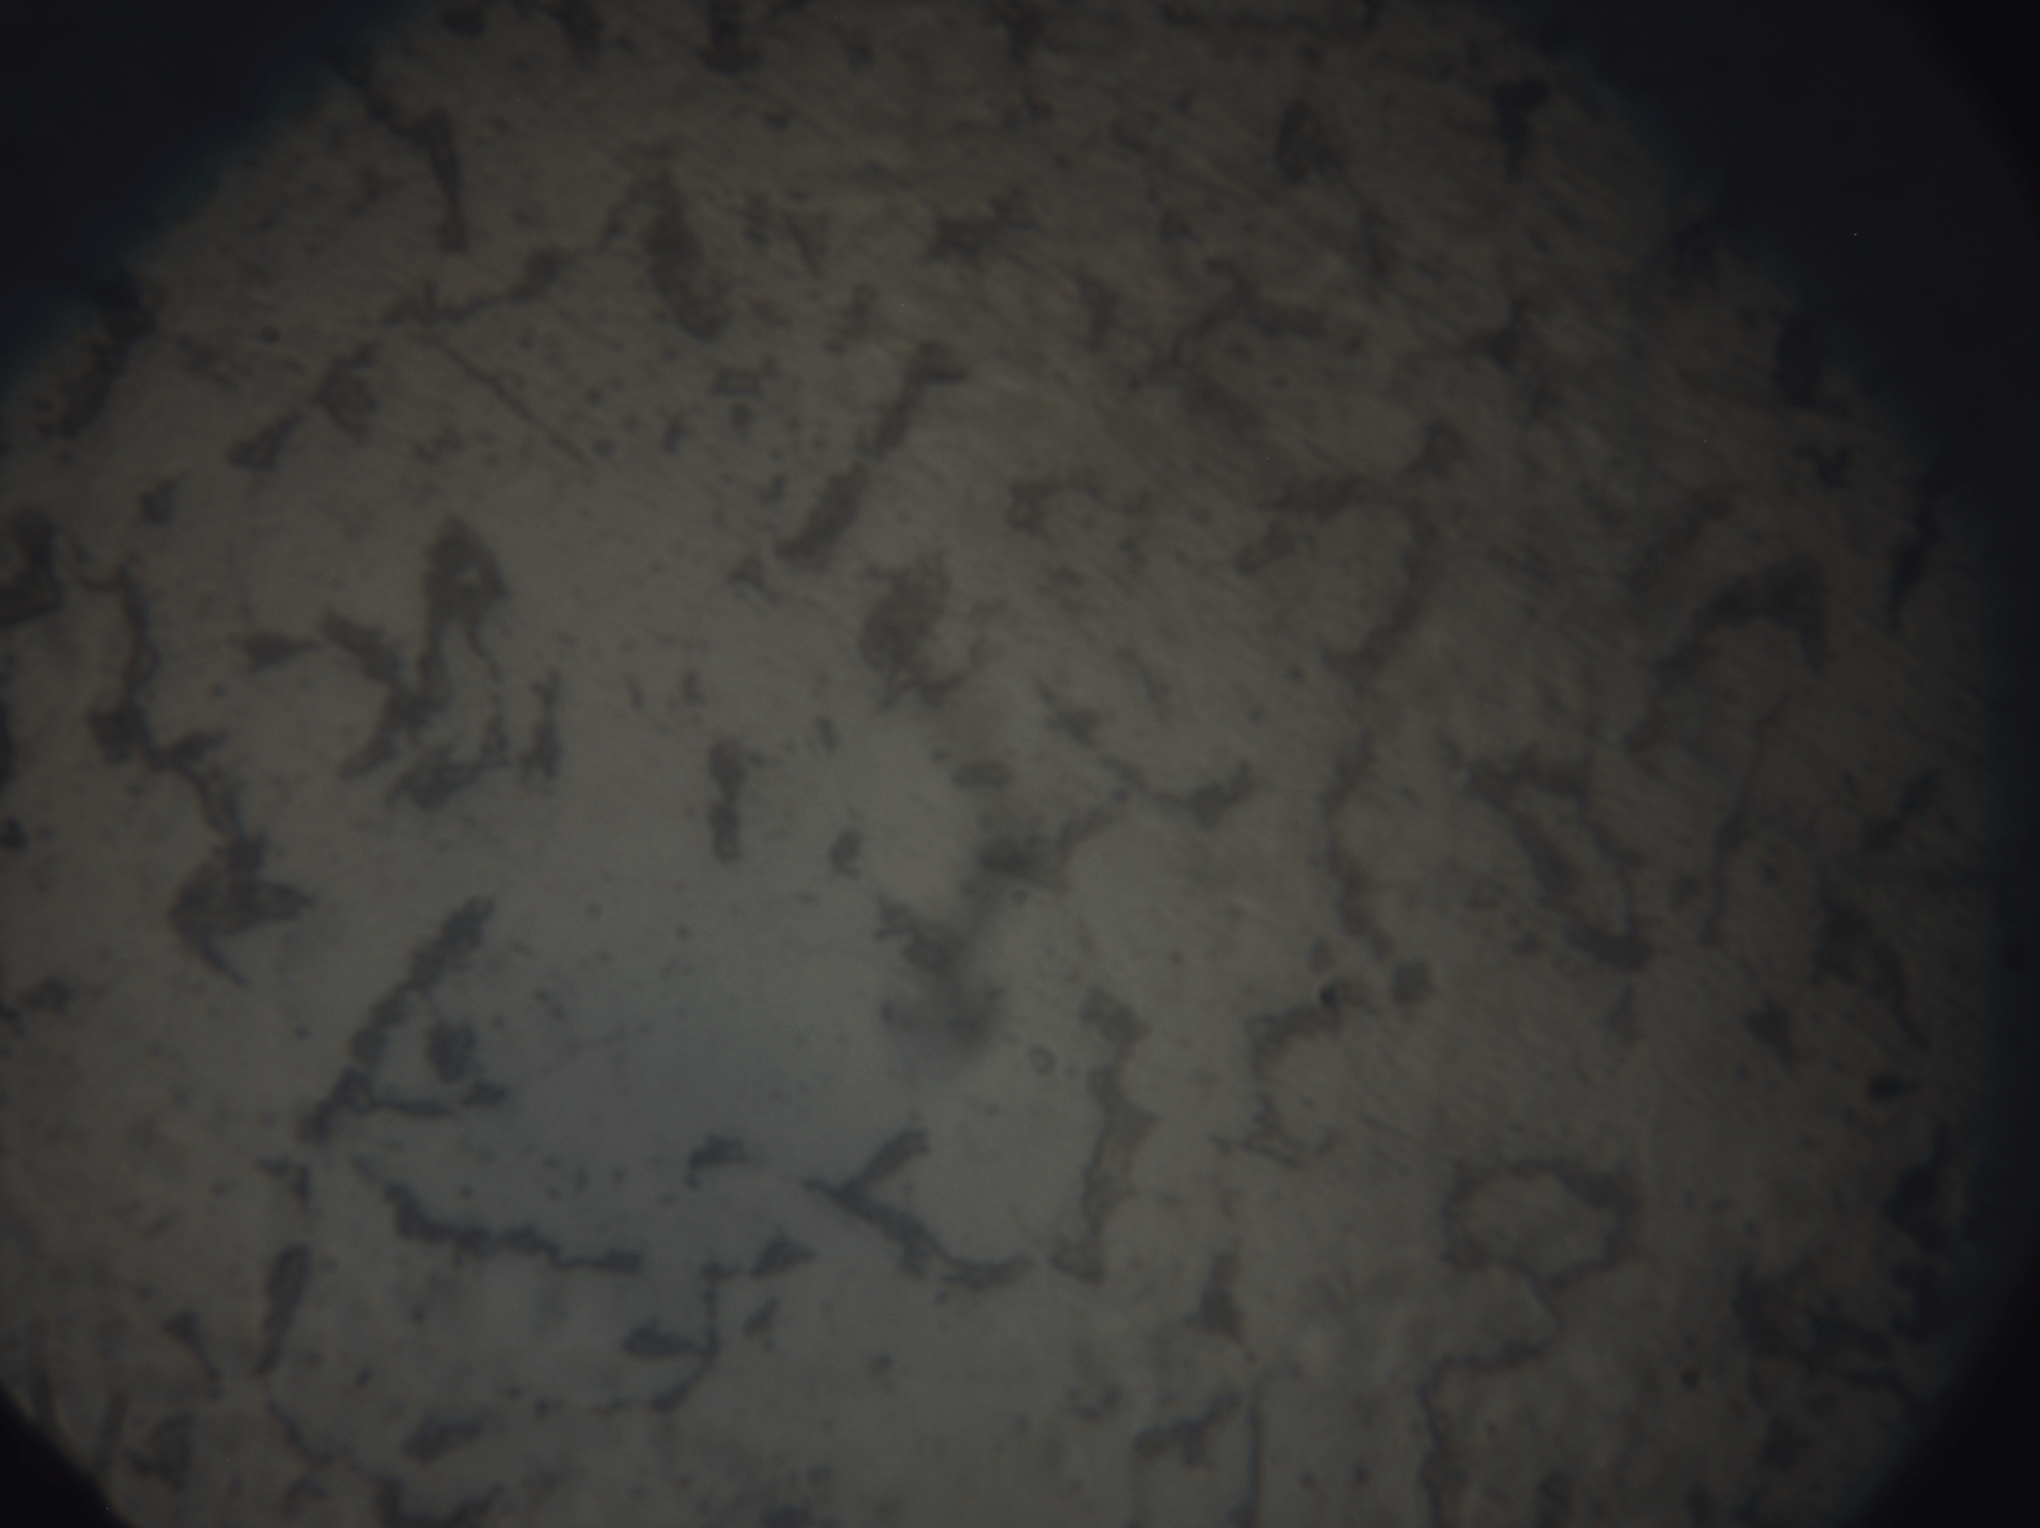
\includegraphics[width=\linewidth]{Figuras/Del-Rio_8.png}
        \caption{Acero IRAM 1020 1000x.}
        \label{1000x}
    \end{subfigure}
    \caption{Micrografías hechas en el Laboratorio de Materiales.}
    \label{fig:metalografia}
\end{figure}

\section{Resolución}
Usando la ecuación de Hall-Petch, resultados experimentales y el diámetro que sacamos anteriormente podemos resolver y sacar las constantes $\sigma_0$ y $k$. Los datos experimentales los obtuvimos de un estracto del trabajo de Z.G. Yang, profesor de la Universidad de Tsinghua (\url{https://www.researchgate.net/publication/257685788_Third_generation_high_strength_low_alloy_steels_with_improved_toughness}).
\begin{equation}
    \sigma_y = \sigma_0 +k\cdot d \textsuperscript{-1/2}
\end{equation}

Los datos que tomamos para sacar las constantes son:
\begin{itemize}
    \item$\sigma_1=$ \SI{1 150}{\mega\pascal}
    \item\(d_1 \textsuperscript{-1/2}=0,75\: \mu m\textsuperscript{-1/2}\)
    \item$\sigma_2=$ \SI{1 070}{\mega\pascal}
    \item\(d_2 \textsuperscript{-1/2}=0,55\: \mu m\textsuperscript{-1/2}\)
\end{itemize}

con los cuales podemos obtener las constantes al remplazar en la ecuación de Hall-Petch.
\begin{equation}
    \sigma_1 = \sigma_0 +k\cdot d_1 \textsuperscript{-1/2}
\end{equation}

\begin{equation}
    \sigma_2 = \sigma_0 +k\cdot d_2 \textsuperscript{-1/2}
\end{equation}

\begin{equation}
    \sigma_0 = \sigma_1 -k\cdot d_1 \textsuperscript{-1/2}
\end{equation}

\begin{equation}
    \sigma_2 = \sigma_1 -k\cdot d_1 \textsuperscript{-1/2} +k\cdot d_2 \textsuperscript{-1/2}
\end{equation}

\begin{equation}
    k = \frac{\sigma_2 - \sigma_1}{d_2 \textsuperscript{-1/2} - d_1 \textsuperscript{-1/2}}
\end{equation}

\begin{equation}
    k = \frac{\SI{1 070}{\mega\pascal} - \SI{1 150}{\mega\pascal}}{{0,55\: \mu m\textsuperscript{-1/2}} - 0,75\: \mu m\textsuperscript{-1/2}}
\end{equation}

\begin{equation}
    k = 380,95\: \text{MPa}\cdot \mu m\textsuperscript{1/2}
\end{equation}

\begin{equation}
    \sigma_0 = \SI{1 150}{\mega\pascal} - 380,95\: \text{MPa}\cdot \mu m\textsuperscript{1/2} \cdot 0,75\: \mu m\textsuperscript{-1/2}
\end{equation}

\begin{equation}
    \sigma_0 = \SI{861,2}{\mega\pascal} 
\end{equation}

Teniendo $\sigma_0$ y $k$ ya ponemos calcular la fluencia de la pieza analizada.

\begin{equation}
    \sigma_y = \SI{861,2}{\mega\pascal} + 380,95\: \text{MPa}\cdot \mu m\textsuperscript{1/2} (116,84\: \mu m)\textsuperscript{-1/2}
\end{equation}
\begin{equation}
    \sigma_y = \SI{896,44}{\mega\pascal} 
\end{equation}

\section{Soldabilidad de los materiales.}
En esta parte veremos la soldabilidad de los distintos materiales de la pieza empleando las expresiones de la American Welding Society
(AWS) y del Instituto Internacional de Soldadura (IIW).\\
primero tenemos que saber las composiciones de los distintos materiales.
\begin{table}[h]
    \centering
    \caption{Composicion de los materiales}
    \begin{tabular}{l|c|c|c}
        \hline
        Composicion & material 1 & material 2 & material 3\\
        \hline
        C & 0,455 & 0,2 & 0,1\\
        Mn & 0,745 & 0.45 & 1,11\\
        Si & 0,231 & 0,225 & 0,72\\
        Cr & 0,041 & 0 & 0\\
        Ni & 0,037 & 0 & 0\\
        Mo & 0,007 & 0 & 0\\
        \hline
    \end{tabular}
\end{table}
Para medir la soldabilidad de un material nos basamos en el contenido de \textbf{carbono equivalente} (\textbf{CE}), que sirve para comprender como los diferentes elementos aleantes aumentan la dureza del material, la cual puede provocar el agrientamiento en frio inducido por hidrogeno.
Pero no todos los aleantes afectan por igual a la dureza por los cuales se crearon relaciones que igualan el impacto de cada elemento a la dureza segun su concentracion.
Y ahora utilizamos las expresiones del AWS y el IIW las cuales son:\\
\subsubsection{AWS:}
\begin{equation*}
    CE = \text{\%C} + \frac{\text{\%Mn}+\text{\%Si}}{6} + \frac{\text{\%Cr}+\text{\%Mo}+\text{\%V}}{5} + \frac{\text{\%Cu}+\text{\%Ni}}{15}
\end{equation*}
La AWS establece que para un contenido de carbono equivalente superior al 0,40\% existe la posibilidad de que se produzcan grietas en la zona afectada por el calor 

\subsubsection{IIW:}
\begin{equation*}
    CE = \text{\%C} + \frac{\text{\%Mn}}{6} + \frac{\text{\%Cr}+\text{\%Mo}+\text{\%V}}{5} + \frac{\text{\%Cu}+\text{\%Ni}}{15}
\end{equation*}
Para medir la soldabilidad la IIW establece un rango de valores de \textbf{carbono equivalente} los cuales son:

\begin{table}[h]
    \centering
    \caption{Rango de valores de CE}
    \begin{tabular}{l|c}
        \hline
        \textbf{Carbon equivalent (CE)} & \textbf{Soldabilidad} \\ \hline
        Hasta 0.35 & Excelente \\ \hline
        0,36--0,40 & Muy bien. \\ \hline
        0,41--0,45 & Bien. \\ \hline
        0,46--0,50 & Feria \\ \hline
        Más de 0,50 & Pobre \\ \hline
    \end{tabular}
\end{table}


\subsection{Soldabilidad de los materiales metodo AWS:}
\subsubsection{Material 1}
\begin{equation*}
    CE = 0,455 + \frac{0,745 + 0,231}{6} + \frac{0,041 + 0,007}{5} + \frac{0,037}{15}
\end{equation*}
\begin{equation*}
    CE = 0,63
\end{equation*}
Teniendo esa cantidad de carbono equivalente existe la posibilidad que se formen grietas en las zonas afectadas por el calor.

\subsubsection{Material 2}
\begin{equation*}
    CE = 0,2 + \frac{0,45 + 0,225}{6} 
\end{equation*}
\begin{equation*}
    CE = 0,3125
\end{equation*}
Teniendo en cuenta la cantidad de carbono equivalente el acero 1020 tiene buena sol

\subsubsection{Material 3}
\begin{equation*}
    CE = 0,1 + \frac{1,11 + 0,72}{6} 
\end{equation*}
\begin{equation*}
    CE = 0,405
\end{equation*}


\subsection{Soldabilidad de los materiales metodo IIW:}
\subsubsection{Material 1}
\begin{equation*}
    CE = 0,455 + \frac{0,745}{6} + \frac{0,041 + 0,007}{5} + \frac{0,037}{15}
\end{equation*}
\begin{equation*}
    CE = 0,59
\end{equation*}

\subsubsection{Material 2}
\begin{equation*}
    CE = 0,2 + \frac{0,45}{6} 
\end{equation*}
\begin{equation*}
    CE = 0,275
\end{equation*}

\subsubsection{Material 3}
\begin{equation*}
    CE = 0,1 + \frac{1,11}{6} 
\end{equation*}
\begin{equation*}
    CE = 0,285
\end{equation*}

\subsection{conclucion}
Teniendo en cuenta el metodo del AWS el material 1 y 2 tienen una soldabilidad baja y pueden llegar a aparecer grietas y presentar fragilidad en las zonas afectadas por el calor.
Y para el material 2 la soldabilidad es mejor que los anteriores al tener un carbono equivalente dentro del limite aceptable.

Y segun el metodo del IIW el material 1 tiene una soldabilidad muy pobre y los materiales 1 y 3 tienen una muy buena soldabilidad.

Segun el reglamento CIRSOC-304, que habla sobre soldadura de aceros en estructuras, y la tabla A.IV-2 que muestra la velocidad de enfriamiento maxima segun para cierta dureza critica, alcanzable en la zona afectada por el calor en la soldadura, segun el porcentaje de \textbf{CE}. la cual nos muestra que el material 2 y el tres no llegan a ninguna de las durezas criticas con las velocidades de la tabla lo que muestra su buena soldabilidad, encabio el material 3 si llega a una dureza critica con una velocidad de enfriamiento de 9$C/s$ por lo que de no tener un precalentamiento a alta temperatura y posible poscalentamiento, la zona afectadas por el calor en el material 1 se volverian muy fragiles.

y esto se puede observar en la macrografía de la pieza donde las zonas cercanas al cordon de soldadura en el material 1, las zonas afectadas por el calor, se encuentran de un color distinto al resto del material de la pieza, en donde es posible que el material se haya fragilizado al no contar con un precalentamiento.

\subsection{Parametro critico del metal (Pcm)}
El Pcm es al igual que las ecuaciones del IIW y la AWS sirve para calcular el carbono equivalente, pero se usa especificamente para aceros donde el porcentaje de carbono no excede el 0,11\% y usualmente se usa en la fabricacion de tuberias

Su ecuacion es:
\begin{equation}
    P_{cm} = \text{\%C} + \frac{\text{\%Si}}{30} + \frac{\text{\%Mn}+\text{\%Cu}+\text{\%Cr}}{20} + \frac{\text{\%Ni}}{60} + \frac{\text{\%Mo}}{15} + \frac{\text{\%V}}{10} + \text{5B\%}
\end{equation}

\section{Calculo de dureza Brinell}

A la hora de trabajar con aceros tener el dato de la dureza Brinell (HB) es muy util debido a que con el se puede obtener de forma aproximada la resistencia a la traccion del material con en el que estamos trabajando, 
lo cual es muy util ya que hacer un ensayo de dureza es mas sencillo y rapido que hacer un ensayo de traccion.

\subsection{Modelos empíricos:}

\begin{equation}
    \sigma_y = X \cdot \text{HB}
\end{equation}

Siendo $X$ la constante de conversion que en este caso para un acero al carbono es 0,36.


\section{Deslizamiento de bordes de grano y de dislocaciones: }

El endurecimiento por Hall-Petch se presenta debido a que al hacerse mas pequeños los granos de un material metalico, aumenta la densidad de bordes de grano y por ende aumenta la cantidad de dislocaciones retenidas en los mismos y se detiene el principal mecanismo de deformación de los metales provocando un aumento de su resistencia a la fluencia y a la traccion (sobretodo el primero al volverse menos ductil el material), pero llegados a un diámetro de grano de 10 nanómetros, los bordes de granos se desplazan, perdiendo parte de la resistencia obtenida la restringir a los desplazamientos de dislocaciones.

En nuestra muestra no se observa el fenome de deslizamiento de borde de grano debido a que nos encontramos con un diametro promedio de grano de \SI{116,84}{\micro\metre} por lo que nos encontramos bastante lejos del tamaño necesario para poder que se de este fenomeno, aparte de que de haber, se necesitaria de un microscopio electronico para poder observarlo con exactitud.

En cambio con las dislocaciones pasa algo distintos y es que defitivamente deben de haber dislocaiones en nuestra muestra, y se podrian ver de haber aplicado el agente corrosivo correcto y se hubiese utilizado un microscopio electronico, debido a que las dislocaciones al igual que los bordes de grano son lugares con mucha energia libre lo cual facilita su corrosion y permite visualizarlo, pero no es caso en este trabajo.
pero se puede asegurar de que hay dislocaciones en la muestra sobretodo al tratarse de una soldadora donde el calor y enfriamiento repentino haya provocado el desplazamiento de las misma.


\end{document}
